\chapter{Implementatie van de monitor}
{\samenvatting Deze masterproef maakt een monitoringsservice met een bijhorende monitoringsAPI die de monitoringsinformatie beschikbaar stelt. De API houdt de resultaten bij in een databank. Deze databank bevat de configuratiegegevens, de resultaten en de beschrijvingen van de verschillende testen. De API doorloopt voor elke aanvraag een opeenvolging van stappen. Zo wordt eerst de aanvraag geparset, vervolgens wordt een query gemaakt en uitgevoerd. Het resultaat van deze query wordt omgevormd tot objecten die vervolgens ge\"encodeerd worden. De website zal deze ge\"encodeerde objecten eerste decoderen en vervolgens visualiseren. Het laatste project is de monitoringsservice. Deze service zal via de API de testen binnenhalen. Deze testen worden vervolgens uitgevoerd en het resultaat wordt teruggestuurd naar de API. Tenslotte is er ook de loadtest die gebruikt wordt om te kijken welke belasting een testbed aankan.}
\clearpage
\section{Databank}
\npar
De databank bestaat uit meerdere tabellen die met elkaar verbonden zijn:
\begin{enumerate}
\item users: deze tabel houdt info bij over de login gegevens die gebruikt worden.
\item testbeds: deze tabel houdt info bij over de testbeds die gemonitord worden.
\item testDefinitions: deze tabel bevat beschrijvingen van de verschillende testen.
\item parameterDefinitions: deze tabel bevat per rij een beschrijving van een parameter.
\item returnDefinitions: deze tabel bevat een beschrijving van de waarden die teruggegeven worden. 
\item testInstance: deze tabel bevat een object van een testDefinitie.
\item parameterInstance: de waardes van de parameters.
\item results: de resultaten
\item subResults: de tussenresultaten.
\end{enumerate}
\npar
Dit alles is geschetst in Figuur \ref{structDatabase} op volgende pagina. Hier zijn de tabellen gegroepeerd op basis van functionaliteit om een beter overzicht te behouden.
\mijnfiguur{width=1\textwidth}{structDatabase}{De stuctuur van de databank}
\clearpage
\subsection{Definities}
\npar
De eerste groep tabellen bevat de definities. De definities bevatten een omschrijving van een test. Hierbij worden de parameters en de tussenresultaten ook opgeslagen. Deze worden opgenomen in een extra tabel om meer flexibiliteit toe te laten. Door de parameters en tussenresultaten in een andere tabel onder te brengen, is het mogelijk om verschillende testen met een variabel aantal tussenresultaten en parameters op te slaan.
\subsection{Instanties}
\npar
Deze tabel houdt de testinstanties bij. Een testinstantie is de test zelf. Als de vergelijking met objectgeori\"enteerd programmeren gemaakt wordt, dan is een testDefinitie een klasse zelf en de instance is dan een object. Deze opsplitsing heeft het voordeel dat de beschrijving van een test apart opgeslagen kan worden. Het is vervolgens zeer eenvoudig om meerdere instanties aan te maken. Ook laat het systeem de nodige flexibiliteit toe om nieuwe definities aan te maken. Net zoals bij de definities zijn de ingevulde waarden hier ook ondergebracht in een aparte tabel. Dit is om dezelfde reden, namelijk het toelaten van een variabel aantal parameters.
\subsection{Configuratiegegevens}
\npar
De configuratiegegevens bestaan uit de gebruikers en de testbeds. De gebruikers zijn belangrijk omdat ze de logininformatie bevatten die gebruikt worden door de automated tester om testen uit te voeren. Zo heeft een logintest een gebruiker nodig die de juiste rechten heeft op dat testbed.
Naast de gebruikers is er ook de informatie over de testbeds. De testbeds hebben o.a. elke een eigen url, urn en naam. Deze informatie wordt in deze tabel ondergebracht. Zowel een gebruiker als een testbed kan/kunnen vervolgens opgegeven worden als een parameter van een testinstance. 
\subsection{Resultaten}
\npar
Deze tabel houdt alle resultaten bij. Elk resultaat heeft een bijhorende logfile; deze wordt momenteel niet opgeslagen in de databank, maar wel apart als file georganiseerd in mappen op harde schijf. Het pad naar de logfile wordt vervolgens opgenomen in de databank. Dit heeft als voordeel dat de databank niet overvol geraakt met logfiles. Op die manier kunnen bijvoorbeeld alle tussenresultaten 6 maanden bijgehouden worden terwijl de logfiles maar voor 2 maanden bijgehouden worden.
\clearpage
\section{Webservice / API}
\npar
De webservice haalt informatie uit de databank op om ze om te vormen naar objecten. Dit verloopt in een aantal fasen, zoals weergegeven in Figuur \ref{structAPI}.
\mijnfiguur{width=1\textwidth}{structAPI}{De werking van de API}
\clearpage
\subsection{Fasen}
\npar
De stappen uit Figuur\ref{structAPI} die doorlopen worden zijn:
\begin{enumerate}
\item parsen van de aanvraag
\item opbouwen van de query
\item uitvoeren van de query
\item samenstellen van de objecten
\item encoderen van de objecten
\end{enumerate}
De tekst hieronder zal kort een overzicht geven van elke stap.
\subsection{Parsen aanvraag}
\npar
Er zijn drie soorten aanvragen. De eerste behandelt het opvragen van configuratiegegeven. De tweede en derde soort zorgen voor het ophalen en toevoegen van resultaten. De laatste groep aanvragen is noodzakelijk voor de monitoringsservice en betreft het ophalen van testen en aanpassen van de planning. Een lijst van alle aanvragen met bijhorende parameters is terug te vinden in bijlage \ref{REFERENCE}.

\npar
Aanvragen van de eerste groep zijn:
\begin{enumerate}
\item testbed: geeft informatie weer over een of meerdere testbeds.
\item user: geeft informatie weer over een of meerdere users.
\item testDefinition: geeft informatie weer over de opbouw van een test.
\item testInstance: geeft informatie weer over de testen.
\end{enumerate}

De tweede groep gaat over het opvragen van resultaten:
\begin{enumerate}
\item last: geeft de laatste resultaten weer.
\item list: geeft een lijst met resultaten weer.
\item q: wordt gebruikt voor het afhandelen van GENI aanvragen. Hierbij wordt de aanvraag ge\"encodeerd in JSON, het antwoord wordt ge\"encodeerd volgens GENI dataschema's (zie ook de referentie in bijlage \ref{REFERENCE}).
\end{enumerate}

\clearpage
Een derde groep aanvragen verzorgt het uitvoeren van de testen en de planning van testen. Bij de planning is vooral het veld nextrun van belang. Dit veld geeft aan wanneer de test een volgende keer uitgevoerd moet worden.
\begin{enumerate}
\item testInstance gefilterd op nextrun: geeft de testen weer die uitgevoerd moeten worden op een zeker tijdsstip.
\item updateNextrun: zal het moment waarop de volgende test uitgevoerd moet worden aanpassen.
\item addResult: zal een nieuw resultaat toevoegen aan de databank hiervoor met het type wel een HTTP-post request zijn.
\end{enumerate}

\subsection{Aanmaken query}
\npar 
In deze stap wordt de query aangemaakt; opgegeven filters worden vertaald naar SQL syntax. Bijvoorbeeld:
\begin{lt}
/last?testdefinitionname=ping,stitching
\end{lt}
zal vertaald worden naar een where clause :
\begin{lt}
... where testdefinitionname IN (ping,stitching) ...
\end{lt}
\npar
Dit wordt gedaan door de QueryBuilder, een interface die verschillende implementaties heeft om verschillende types van aanvragen te behandelen. Zo wordt een aanvraag afkomstig van GENI door een andere queryBuilder afgehandeld dan een aanvraag van binnen FIRE.

\subsection{Uitvoeren query}
\npar
In deze stap wordt de query uitgevoerd met behulp van de php-pgsql module die de verbinding tussen PHPcode en een postgreSQL databank afhandelt.
\clearpage
\subsection{Samenstellen van objecten}
\npar
In deze stap wordt het resultaat van de query lijn per lijn overlopen en worden objecten gevormd. Om compabiliteit te verhogen worden er geen klassen zoals testbed, user en test aangemaakt, maar wordt alles direct opgeslagen in geneste array\footnote{Merk op dat een PHP array zowel een map als een array is.}. Een geneste array is een array die arrays bevat. Deze arrays kunnen op hun beurt weer bestaan uit arrays en zo verder. 
\npar
Deze manier van werken spaart tijd. De objecten worden direct in de 'vorm' van het dataschema gegoten. Een dataschema is een definitie van de vorm van het antwoord; concreter: hoe het antwoord er zal uitzien. Dit wordt gedaan door de fetcher. Opnieuw wordt hier gebruik gemaakt van overerving om andere dataschema's te ondersteunen.
\subsection{Encoderen van objecten}
\npar
De encodering is de laatste stap die het mogelijk maakt om objecten te versturen over een netwerk. De encodering wordt gedaan in JSON door de formatter. Door overerving kan hier gemakkelijk gezorgd worden voor extra coderingen bijvoorbeeld xml-encodering.
\section{Website}
\npar
De website bestaat uit een aantal verschillende interfaces waarvan de eerste de FLS (First Level Support) monitor is. Deze heeft als doel om voor elk testbed een snelle, eenvoudige statusweergave te voorzien. Een screenshot is te zien in Figuur \ref{flsnieuw}.
\mijnfiguur{width=1\textwidth}{flsnieuw}{FLS monitor}
\clearpage
\npar
Een volgende interface wordt gebruikt om detailresultaten weer te geven voor \'e\'en testtype. In Figuur \ref{loginnieuw} wordt een overzicht gegeven van de login testen\footnote{Login2 in de titel is te verklaren omdat dit logintesten zijn die met de aggregate manager versie 2 werken.}. Op deze figuur kan eenvoudig afgelezen worden dat de test voor het eerste testbed mislukt is en dat de oorzaak daarvan bij stap twee en vier (in rood) ligt. Diezelfde test is wel gelukt voor wall1 en wall2, maar met een waarschuwing bij stap 5.
\mijnfiguur{width=1\textwidth}{loginnieuw}{Overzicht van resultaten van de login testen.}
\npar
Tenslotte is er nog een overzicht van de geschiedenis van een specifieke test. Dit is zichtbaar in Figuur{histnieuw}. Wanneer de cursor over een tussenresultaat gaat, verschijnt er een tooltip\footnote{Maakt gebruik van powertip, beschikbaar op http://stevenbenner.github.io/jquery-powertip/} waarop de naam van de subtest samen met de status wordt weergegeven\footnote{Dit is ook mogelijk bij de weergave van een test.}.
\mijnfiguur{width=1\textwidth}{histnieuw}{Geschiedenis van een login test.}
\npar 
Bij elke test is het mogelijk om de console-uitvoer te bekijken, deze is beschikbaar in de log. Naast de console-uitvoer genereert de automated tester ook een XML en HTML file met informatie over het verloop van de test. Deze zijn ook beschikbaar, zie Figuur \ref{overviewxml} en Figuur \ref{overviewhtml}.
\begin{figure}[H]
\centering
\begin{subfigure}{.45\textwidth}
  \centering
  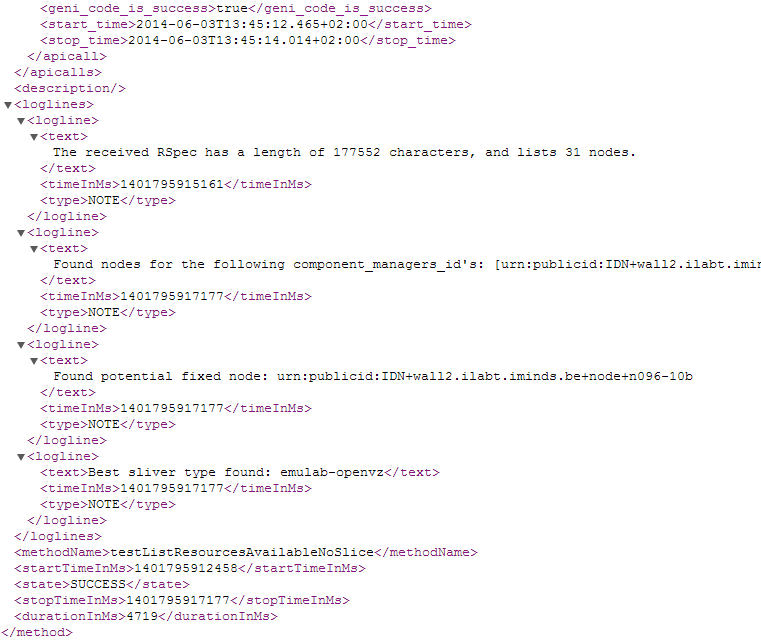
\includegraphics[width=.9\textwidth]{overviewxml}
  \caption{\label{overviewxml} De originele overview in XML formaat}
\end{subfigure}
\begin{subfigure}{.45\textwidth}
  \centering
  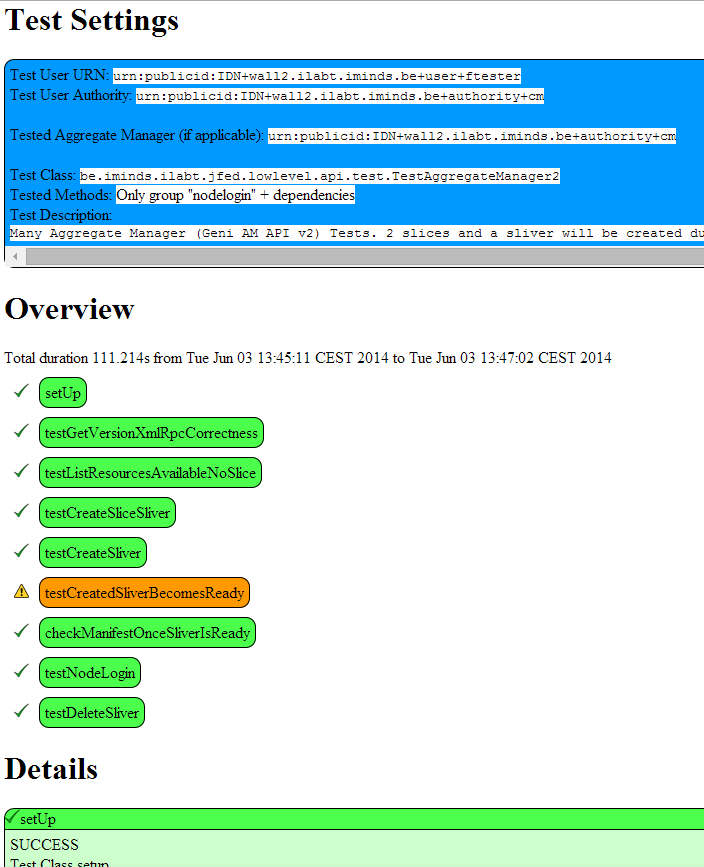
\includegraphics[width=.9\textwidth]{overviewhtml}
  \caption{\label{overviewhtml}Overview in html formaat}
\end{subfigure}
\caption{Naast de console uitvoer zijn ook het originele resultaat in XML formaat en het overeenkomstige HTML formaat beschikbaar.}
\end{figure}

\section{Service}
\npar
De service werkt met meerdere threads. Er is \'e\'en hoofdthread die testen ophaalt via de API en deze toevoegt aan een queue. Vervolgens worden de testen \'e\'en voor \'e\'en uit de queue gehaald en uitgevoerd door de threadpool. De grootte van de threadpool is instelbaar. Standaard is dit $cpu_{cores} * 2 + 1$.
\npar
Elke test wordt uitgevoerd op een aparte thread. Tijdens de uitvoering wordt verbinding gemaakt met \'e\'en of meerdere testbeds via de jFed automated tester. Deze geeft een XML-file terug waaruit de tussenresultaten geparset worden. Deze resultaten worden vervolgens doorgegeven aan de resultuploader.
\npar
De resultuploader staat in voor het doorsturen van resultaten naar de API en draait op een aparte thread. Hierbij wordt ook de volgende uitvoeringstijd aangepast. Dit proces wordt beschreven in Figuur \ref{structService}.
\mijnfiguur{width=1\textwidth}{structService}{De werking van de monitoringsservice}


\clearpage

\section{Loadtest}
\subsection{Uitwerking}
\npar
De uitwerking wordt weergegeven in Figuur \ref{structLoadtest}. Let op de overeenkomsten met Figuur \ref{structService}, waar de monitoringsservice wordt uitgelegd. De uitwerking van de loadtest is op een aantal stappen na, gelijk aan de uitwerking van de monitoringsservice, vermits de kern van beide gelijk is. 
\npar
Eerst wordt de bestaande test opgehaald. Daarna wordt een threadpool aangemaakt met de grootte n; het aantal testen dat uitgevoerd moet worden. Hierdoor kunnen alle testen tegelijkertijd uitgevoerd worden. Vervolgens wordt elke test opgestart na een instelbaar interval. Dit interval zorgt er bijvoorbeeld voor dat de testen elkaar om de 2 seconden opvolgen.
\npar
Eenmaal een test is opgestart en uitgevoerd, wordt elk resultaat geparset en doorgegeven aan de resultuploader. Deze zal de resultaten \'e\'en voor \'e\'en uploaden en daarbij de uitvoeringstijd van de volgende test niet aanpassen. Dat laatste zou ertoe leiden dat volgende resultaten niet meer aanvaard worden. Merk het verschil met de monitoringsservice die hier wel een aanpassing doet van het nextrun veld, zie ook bijlage \ref{ONDERHOUD}. Dit veld houdt bij wanneer de test een volgende keer uitgevoerd wordt.
\npar
Na het uitvoeren van de testen zijn de resultaten van de stresstest beschikbaar via de monitoringsAPI. De huidige implementatie maakt geen onderscheid tussen resultaten van de monitoringsservice en de loadtesten. In plaats daarvan wordt de databank samen met de API gekloond. De resultaten zijn beschikbaar in de gekloonde databank, die na elke stresstest gewist wordt om de resultaten overzichtelijk te houden. Samenvoegen van de monitoringresultaten met de loadtestresultaten is mogelijk, maar bleek noch een prioriteit, noch noodzakelijk te zijn.
\mijnfiguur{width=1\textwidth}{structLoadtest}{De uitwerking van de loadtesten.}
\clearpage
\subsection{Voorbeeld van een stresstest}
\npar
Deze sectie bevat een voorbeeld van een uitgevoerde loadtest als voorbereiding voor een practicum door de Griekse universiteit van Patras. Tijdens dit practicum zullen een 50-tal studenten elk 2 PC's gebruiken om TCP congestion testen. Hierbij zal de virtual wall of wall1 gebruikt worden als testbed. Doordat alle studenten hun experiment op zeer korte tijd van mekaar zullen starten, zal een grote belasting ontstaan op het testbed. Om te kijken of het testbed dergelijke belasting aankan, wordt een loadtest van 119 PC's uitgevoerd. Deze loadtest zal het practicum simuleren en weergeven of er problemen optreden. De loadtest is uitgevoerd met de code die geschreven werd in de masterproef. Het meten van resultaten en weergeven van grafieken is gebeurd door andere tools.
\npar
Figuur \ref{verslag119pcs} geeft een overzicht van de gebruikte computers. Deze computers zijn per twee opgedeeld in slices. Figuur \ref{verslagresources} geeft een overzicht van deze slices met bijhorende status. Op deze figuur komt een groen vak overeen met een slice die gelukt is, een rood vak daarentegen duidt op problemen.
\mijnfiguur{width=1\textwidth}{verslag119pcs}{Overzicht van de verschillende slices.}
\mijnfiguur{width=1\textwidth}{verslagresources}{Status van de slices.} 
\npar
Vermits er in Figuur \ref{verslagresources} maar \'e\'en pc rood is, kan besloten worden dat het testbed dergelijke belasting kan verwerken. Figuur \ref{verslaggrafiek} hieronder geeft een grafiek van de belasting van het testbed op die dag. Uiterst rechts op de figuur zijn er 2 hoge waarden zichtbaar, deze zijn veroorzaakt door de stresstest. Doordat het testbed een dubbel aantal cores ziet dan dat er werkelijk zijn, moeten de percentages verdubbeld worden. De stresstest met 119 computers geeft bijgevolg een belasting van 80\% voor een bepaalde tijd.
\mijnfiguur{width=1\textwidth}{verslaggrafiek}{Belasting van het testbed, percentages moeten verdubbeld worden.} 
\clearpage
\npar
Vervolgens werd de test herhaald met 100 gebruikers die telkens 2 computers gebruiken. De veroorzaakte belasting is te zien in Figuur \ref{verslaggrafiek100users}. Ook hier moeten de percentages verdubbeld worden wat een belasting van 90\% geeft over een langere periode.
\mijnfiguur{width=1\textwidth}{verslaggrafiek100users}{Belasting van een testbed met 100 gebruikers} 
\npar
De test met 100 gebruikers bestaat eigenlijk uit 100 testen die tegelijk draaien. Voor elke test is bijgevolg een resultaat, dat te zien is op de monitoringsinterface\footnote{Deze monitoringsinterface is een kloon van de werkende monitoringsAPI die enkel stresstesten uitvoert.}. Figuur \ref{verslag100} geeft resultaten per test voor 100 users. Het is duidelijk dat er hier en daar problemen optreden, maar dat het overgrote deel wel slaagt.
\npar
Doordat de load veel hoger is dan wat de studenten in werkelijkheid zullen doen is de stresstest succesvol. 
\mijnfiguur{width=1\textwidth}{verslag100}{Weergave per test} 